\documentclass{mynote}

\begin{document}
\section{普遍规律}
\subsection{电场和势}
符号约定
\begin{center}
    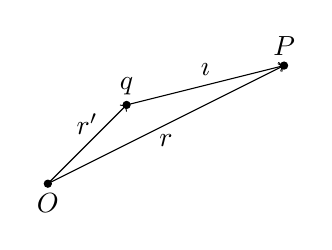
\begin{tikzpicture}
        \fill (0,0) circle (1.5pt) node[below]{$O$};
        \fill (1,1) circle (1.5pt) node[above]{$q$};
        \fill (3,1.5) circle (1.5pt) node[above]{$P$};
        \draw[->] (0,0)--(1,1) node[midway, above]{$\bm{r}'$};
        \draw[->] (1,1)--(3,1.5) node[midway, above]{$\bm{\imath}$};
        \draw[->] (0,0)--(3,1.5) node[midway, below]{$\bm{r}$};
    \end{tikzpicture}
\end{center}

\begin{define}{静电场}
    \[
    \bm{E}(\bm{r}) = \frac{1}{4\pi \varepsilon_0} \sum_{i=1}^n \frac{q_i}{\imath_i^2} \hat{\bm{\imath}}_i    
    \]
    电荷连续分布的情况下有
    \[
    \bm{E}(\bm{r}) = \frac{1}{4\pi \varepsilon_0} \int \frac{\rho (\bm{r}')}{\imath^2} \hat{\bm{\imath}} \dl \tau'
    \]
\end{define}





\begin{theorem}{高斯定律}
    这是电动力学的基本定律之一。
    \[
    \boxed{
    \nabla \cdot \bm{E} = \frac{1}{\varepsilon_0} \rho   } 
    \]
\end{theorem}
\begin{proof}
    电场在环闭曲面的积分与曲面形状无关。这一点可以从高斯定理定义得出:
    \[
    \int_{\mathcal{S}} \bm{f} \cdot \dl \bm{a} = \int_{\mathcal{V}} \nabla \cdot \bm{f} \dl \tau    
    \]
    所以不妨直接让曲面是一个球,考虑静电场的情况,有
    \[
    \oint_{\mathcal{S}} \bm{E}\cdot \dl \bm{a} = \frac{1}{4\pi \varepsilon_0} \int \frac{q}{r^2} \hat{\bm{r}} \cdot r^2 \hat{\bm{r}} \sin \theta \dl \theta \dl \phi  = \frac{q}{\varepsilon_0}  
    \]
    带入高斯公式
    \[
    \nabla \cdot \bm{E} = \frac{1}{\varepsilon_0} \rho    
    \]
\end{proof}





\begin{proposition}
    \[\nabla \times \bm{E} = 0\]
\end{proposition}
\begin{proof}
    $\dl \bm{l} = \dl r \hbm{r} + r \dl \theta \hbm{\theta} + r \sin \theta \dl \phi \hbm{\phi}$,注意到$\hbm{r},\; \hbm{\theta} ,\; \hbm{\phi}$在一点处是正交的,则
    \[
    \bm{E} = \frac{1}{4\pi \varepsilon_0} \frac{q}{r^2} \hbm{r}    
    \]
    有
    \[
    \bm{E} \cdot \dl \bm{l} = \frac{1}{4\pi \varepsilon_0} \frac{q}{r^2} \dl r    
    \]
    于是
    \[
    \int_a^b \bm{E} \cdot \dl \bm{l} = \frac{1}{4\pi \varepsilon_0} \left( \frac{q}{r_a} - \frac{q}{r_b} \right)    
    \]
    因此
    \[
    \oint \bm{E} \cdot \dl \bm{l} = 0    
    \]
\end{proof}




\begin{define}{电势}
    \[
    \bm{E} = - \nabla V    
    \]
    在一条路径上选定一个参照点$\mathcal{O}$,可以定义一个函数
    \[
    V(r) = \int^r_{\mathcal{O}} \bm{E} \cdot \dl \bm{l}    
    \]
    得到
    \[
    V(b) - V(a) = -\int_a^b \bm{E} \cdot \dl \bm{l}
    \]
    考虑原函数
    \[
    V(b) - V(a) = \int_a^b \nabla V \cdot \dl \bm{l}
    \]
    所以得到电势的定义。这里和理论力学的教材不一致,后者是$F = -\nabla V$。
\end{define}





\subsection{电流和磁场}
\begin{define}{0}
    各种定义

    \begin{itemize}
        \item 电流$\bm{I}$:单位时间垂直通过某一面积的电荷量。
        \item 电流密度$\bm{J}$:单位时间垂直通过单位面积的电荷量。
        \item 电极化强度$\bm{P}$:穿过单位面积的正电荷量,电流密度可用$\pp{\bm{P}}{t}$刻画。
    \end{itemize}
\end{define}


\begin{theorem}{电荷守恒}
    这是物理学大厦的基本定律之一。
    \[
    \boxed{
        \nabla \cdot \bm{J} = -\pp{\rho}{t}    
    }    
    \]
\end{theorem}
\begin{proof}
    \[
        \oint_{\mathcal{S}} \bm{J} \cdot \dl \bm{S} = -\int_{\mathcal{V}} \pp{\rho}{t} \dl \tau \Leftrightarrow \nabla \cdot \bm{J} = -\pp{\rho}{t}    
    \]
\end{proof}
在恒定电流下$\pp{\rho}{t}=0$,导致$\nabla \cdot \bm{J} = 0$,不恒定一般没有这种情况。





\begin{theorem}{毕奥萨伐尔定律}
    电动力学的基础公式之一。
    \[
    \boxed{
    \bm{B}(\bm{r}) = \frac{\mu_0}{4 \pi} \int_{\mathcal{V}} \frac{\bm{J}(\bm{r}') \times \bm{\imath}}{\imath^3} \dl \tau'    }
    \]
    实际上$\bm{J} \dl \tau'$应当是矢量,$\bm{J}$与$\dl \bm{l}$方向相同,并且$\dl \tau' = \dl \bm{S} \cdot \dl \bm{l}$,易证$\bm{J} \dl \bm{S} \cdot \dl \bm{l} = \bm{J}  \cdot  \dl \bm{S} \dl \bm{l} $,在恒定电流下
    \[
        \frac{\mu_0}{4 \pi} \int_{\mathcal{V}} \frac{\bm{J}(\bm{r}') \times \bm{\imath}}{\imath^3} \dl \tau'  = \frac{\mu_0}{4 \pi} \int_{L} \frac{I \dl \bm{l} \times \bm{\imath}}{\imath^3}
    \]
\end{theorem}
\begin{problem}{一个粒子}
    无限长导线,电流恒定,求半径$r$处的磁感应强度。
\end{problem}
\begin{solution}
    选择夹角$\theta$作为参数,选择平面直角坐标系。
    \[
    \bm{r}' = (0, 0, r \tan \theta) \quad \bm{r} = (r, 0, 0) \quad \bm{\imath} = (r, 0, - r \tan \theta)
    \]
    \[
    \dl \bm{l} = \dl \bm{r}' = (0, 0, r/\cos^2 \theta \dl \theta) \quad \imath^3 = \left( \frac{r}{\cos \theta} \right) ^3
    \]
    \[
    \bm{B}(r) = \frac{\mu_0}{4 \pi} \int_{-\frac{\pi}{2}}^{\frac{\pi}{2}} \dfrac{r^2 \e_y }{\frac{r^3}{\cos^3 \theta} \cos^2 \theta} \dl \theta  = \frac{\mu_0 I}{2\pi r} \e_y
    \]
\end{solution}






\begin{proposition}
    由毕奥萨伐尔定律的公式可直接推得,过程太复杂省略(P.12.)
    \[
    \nabla \times \bm{B} = \mu_0 \bm{J}
    \]
    上式只在恒定电流下成立,下式始终成立。
    \[
    \nabla \cdot \bm{B} = 0    
    \]
\end{proposition}





\begin{theorem}{电磁感应定律}
    电动势和磁通量的关系
    \[
    \nabla \times \bm{E} = -\pp{\bm{B}}{t}    
    \]  
\end{theorem}
\begin{proof}
    \[
        \epsilon = \oint_L \bm{E} \cdot \dl \bm{l} = -\int_{\mathcal{S}} \pp{\bm{B}}{t} \dl \bm{a}
    \]
\end{proof}




\begin{proposition}
    在恒定电流下$\Rightarrow \nabla \times \bm{B} = \mu_0 \bm{J} \Rightarrow \nabla \cdot (\nabla \times \bm{B}) = \nabla \cdot \mu_0 \bm{J} = 0 \Rightarrow \nabla \cdot \bm{J} = 0$,这与电荷守恒定律$\nabla \cdot \bm{J} = -\pp{\rho}{t}  $不完全一致,需要推广。引入位移电流密度$\bm{J}_D$,使其能满足$\nabla \cdot (\bm{J} + \bm{J}_D) = 0$. 这个操作可以看作在线路断开时,如存在电容时,$\nabla \cdot \bm{J} \ne 0$,但引入辅助量后使其可以视为闭合线路。

    考察
    \[
    \left\{
        \begin{aligned}
            & \nabla \cdot \bm{J} + \pp{\rho}{t} = 0 \\
            & \varepsilon_0 \nabla \cdot \bm{E} = \rho
        \end{aligned} 
    \right.    
    \]
    得到$\nabla \cdot \left( \bm{J} + \varepsilon_0 \pp{\bm{E}}{t} \right) = 0$,自然让$\bm{J}_D = \varepsilon_0 \pp{\bm{E}}{t}$,带入$\nabla \times \bm{B} = \mu_0 \bm{J}'$从而得出
    \[
        \nabla \times \bm{B} = \mu_0 \bm{J} + \mu_0 \varepsilon_0 \pp{\bm{E}}{t}
    \]
\end{proposition}



\begin{theorem}{真空麦克斯韦方程组}
    \[
    \left\{
        \begin{aligned}
            & \nabla \times \bm{E} = -\pp{\bm{B}}{t} \\
            & \nabla \times \bm{B} = \mu_0 \bm{J} + \mu_0 \varepsilon_0 \pp{\bm{E}}{t} \\
            & \nabla \cdot \bm{E} = \frac{\rho}{\varepsilon_0} \\
            & \nabla \cdot \bm{B} = 0
        \end{aligned}
    \right.   
    \]
\end{theorem}





\subsection{极化和磁化}
\begin{theorem}{电极化强度和束缚电荷密度的等同}
    \[
        \nabla\cdot \bm{P} = -\rho_P  
    \]
\end{theorem}
\begin{proof}
    单个分子的电极化强度$\bm{p}$时矢量,定义为电荷量乘以被外场拉开的正负电荷距离矢量$\bm{l}$,即$\bm{p} = q \bm{l}$。宏观极化强度定义为
    \[
    \bm{P} = \dfrac{\sum_i \bm{p}_i}{\Delta V}    
    \]
    分子数密度为$n$,且体积为$\dl \bm{S} \cdot \bm{l}$时,穿出该体积的正电荷数目为$nq\bm{l} \cdot \dl \bm{S}$,它鬼使神差地构成了单位面积的电极化强度通量
    \[
        nq\bm{l} \cdot \dl \bm{S} = n\bm{p} \cdot \dl \bm{S} = \bm{P} \cdot \dl \bm{S}
    \]
    由于正电荷穿出面外,留下了净余负电荷,定义这些负电荷的密度为束缚电荷密度$\rho_P$,求积分得到
    \[
    \oint_{\mathcal{S}} \bm{P}\cdot \dl \bm{a} = -\int_{\mathcal{V}} \rho_P \dl \tau    
    \]
\end{proof}



\begin{proposition}
    在介质分界面处,两边各取一个薄层,假设$\bm{P}_1$为流入的极化强度,$\bm{P}_2$为流出的极化强度。定义束缚电荷面密度$\sigma_P$为分界面单位面积的束缚电荷量。由于极化强度通量等于穿出正电荷数量,得
    \[
    (\bm{P}_2 - \bm{P}_1) \cdot \dl \bm{S} = - \sigma_P \dl S    
    \]
    分解$\dl \bm{S} = \e_n \dl S$,进一步写出
    \[
        (\bm{P}_2 - \bm{P}_1) \cdot \e_n = -\sigma_P
    \]
\end{proposition}



\begin{define}{电位移矢量}
    \[
    \boxed{
        \bm{D} = \varepsilon_0 \bm{E} + \bm{P}
    }    
    \]
    来源于$\varepsilon_0 \nabla \cdot \bm{E} = \rho_f + \rho_P$,而$\rho_P = -\nabla \cdot \bm{P}$,进一步得出
    \[
    \boxed{
        \nabla \cdot \bm{D} = \rho_f
    }    
    \]
\end{define}



\begin{proposition}
    一般各向同性的线性介质满足$\bm{P} = \chi_e \varepsilon_0 \bm{E}$,一般记$\varepsilon = \varepsilon_r \varepsilon_0 ,\; \varepsilon_r = 1+\chi_e$.
\end{proposition}







\begin{theorem}{磁化强度和磁化电流密度的等同}
    \[
        \nabla \times \bm{M} = \bm{J}_M
    \]
\end{theorem}
\begin{proof}
    单个分子的磁偶极矩定义为矢量$\bm{m} = i\bm{a}$,$i$是电流,$\bm{a}$是电流环绕面积,方向为法向。宏观磁化强度定义为
    \[
    \bm{M} = \dfrac{\sum_i \bm{m}_i}{\Delta V}    
    \]
    在一个曲面上,对边界的磁化电流有贡献的仅有边界处的分子们;如果分子数密度为$n$,计算能让边界处于分子电流内的所有数目,等价于计算以边界为轴分子电流半径为半径的圆柱体积再乘以分子数;体积为$V_L = \oint_L \bm{a} \cdot \dl \bm{l}$,分子数为$\oint_L n \bm{a} \cdot \dl \bm{l}$,所以曲面$S$边界处从背面流向正面的总磁化电流为
    \[
    I_M = \oint_L n i \bm{a} \cdot \dl \bm{l} = \oint_L n\bm{m} \cdot \dl \bm{l} = \oint_L \bm{M} \cdot \dl \bm{l}    
    \]
    同时用磁化电流密度表示磁化电流
    \[
    \int_{\mathcal{S}} \bm{J}_M \cdot \dl \bm{a} =    \oint_L \bm{M} \cdot \dl \bm{l}  
    \]
\end{proof}





\begin{proposition}
    电场变化会使电极化强度变化,而这种变化根据定义可以用来刻画极化电流密度。
    \[
    \bm{J}_P := \pp{\bm{P}}{t}    
    \]
    $\pp{\bm{P}}{t}$应该解释为单位时间穿过单位面积的正电荷量,对比电流密度的定义"单位时间垂直通过单位面积的电荷量",如果将$\bm{J}_P$的方向定义为$\bm{P}$的方向,“垂直通过单位平面”的概念消失了。
\end{proposition}
\begin{proof}
    已知
    \[
    \left\{
        \begin{aligned}
            & \nabla \cdot \bm{J} = -\pp{\rho}{t} \\
            & \nabla \cdot \bm{P} = -\rho_P
        \end{aligned} 
    \right.    
    \]
    欲证
    \[
    \bm{J} = \pp{\bm{P}}{t}    
    \]
    由$\nabla \cdot \bm{P} = -\rho_P$推出$\nabla \cdot \pp{\bm{P}}{t} = -\pp{\rho_P}{t} = \nabla \cdot \bm{J}$,所以$\pp{\bm{P}}{t} = \bm{J}$.
\end{proof}





\begin{define}{磁场强度}
    \[
    \boxed{
        \bm{H} = \frac{\bm{B}}{\mu_0} - \bm{M}
    }    
    \]
    来源于$\dfrac{1}{\mu_0} \nabla \times \bm{B} = \bm{J}_F + \bm{J}_M + \bm{J}_P + \varepsilon_0 \pp{\bm{E}}{t}$,且$\bm{J}_M = \nabla \times \bm{M},\; \bm{J}_P = \pp{\bm{P}}{t}$,进一步得到
    \[
    \boxed{
        \nabla \times \bm{H} = \bm{J}_f + \pp{\bm{D}}{t}
    }    
    \]
\end{define}



\begin{proposition}
    最简单的有$\bm{M} = \chi_M \bm{H}$,记$\bm{B} = \mu \bm{H}$,且$\mu = \mu_r \mu_0,\; \mu_r = 1 + \chi_M$.
\end{proposition}








\begin{theorem}{介质麦克斯韦方程组}
    \[
    \left\{
        \begin{aligned}
            & \nabla \times \bm{E} = -\pp{\bm{B}}{t} \\
            & \bcancel{ \dfrac{1}{\mu_0} \nabla \times \bm{B} = \bm{J}_f + \bm{J}_P + \bm{J}_M + \varepsilon_0 \pp{\bm{E}}{t} } \\
            & \nabla \times \bm{H} = \bm{J}_f + \pp{\bm{D}}{t} \\
            & \bcancel{\varepsilon_0 \nabla \cdot \bm{E} = \rho_f + \rho_P } \\
            & \nabla \cdot \bm{D} = \rho_f \\
            & \nabla \cdot \bm{B} = 0
        \end{aligned} 
    \right.    
    \]
\end{theorem}




\subsection{边值关系}
电场或磁场不连续的情况不能使用微分形式的麦克斯韦方程,而改用积分形式。
\[
\left\{
    \begin{aligned}
    & \oint_L \bm{E} \cdot \dl \bm{l} = - \int_{\mathcal{S}} \pp{\bm{B}}{t} \dl \bm{a} & (1) \\
    & \oint_L \bm{H} \cdot \dl \bm{l} = I_f + \int_{\mathcal{S}} \pp{\bm{D}}{t} \dl \bm{a} & (2)\\
    & \oint_{\mathcal{S}} \bm{D} \cdot \dl \bm{a} = Q_f & (3)\\
    & \oint_{\mathcal{S}} \bm{B} \cdot \dl \bm{a} = 0 & (4)
    \end{aligned} 
\right.    
\]



\begin{figure}[H]
    \centering
    \includegraphics[width=2in]{./Imgs/QQ_Image_1664287192148.jpg}
\end{figure}


\begin{proposition}
    考察(3)式, $ \oint_{\mathcal{S}} \bm{D} \cdot \dl \bm{a} = Q_f$,取边界面上极薄的易拉罐,其侧边的通量可忽略不计。于是
    \[
        \oint_{\mathcal{S}} \bm{D} \cdot \dl \bm{a} = - \int_{\Delta S} \bm{D} \cdot \dl \bm{a} + \int_{\Delta S} \bm{D} \cdot \dl \bm{a} = (-\bm{D}_1  + \bm{D}_2) \cdot \Delta \bm{S}
    \]
    (这里似乎还隐含了$\bm{D}$不随坐标而变化,但在界面两端是不一致的),同时$Q_f = \sigma_f \Delta S$
    \[
        (-\bm{D}_1  + \bm{D}_2) \cdot \Delta \bm{S} = \sigma_f \Delta S \Rightarrow (-\bm{D}_1  + \bm{D}_2) \cdot \e_n \Delta S = \sigma_f \Delta S \Rightarrow \boxed{(-\bm{D}_1  + \bm{D}_2) \cdot \e_n = \sigma_f}
    \]
\end{proposition}




\begin{proposition}
    考察(4)式,和上面一样的分析得到
    \[
        (-\bm{B}_1  + \bm{B}_2) \cdot \Delta \bm{S} = 0 \Rightarrow     \boxed{(-\bm{B}_1  + \bm{B}_2) \cdot \e_n = 0}
    \]
\end{proposition}




\begin{figure}[H]
    \centering
    \includegraphics[width=2in]{./Imgs/QQ_Image_1664287190967.jpg}
\end{figure}

\begin{proposition}
    考察(2)式,定义电流线密度$\bm{a}_f$,大小为垂直通过单位横截线的电流大小。任取$\Delta \bm{l}$,$\e_n$与$\Delta \bm{l}$的法线矢量为$\e_n \times \Delta \bm{l}$,故经过$\Delta \bm{l}$的电流为$I_f = (\e_n \times \Delta \bm{l}) \cdot \bm{a}_f$。回到$(\bm{u} \times \bm{v}) \cdot \bm{w} = \epsilon^{\mu \nu \rho} u_{\mu} v_{\nu} w_{\rho} = \epsilon^{\rho \mu \nu} w_{\rho} u_{\mu} v_{\nu} $,相当于经历两次行交换。所以$I_f = (\e_n \times \Delta \bm{l}) \cdot \bm{a}_f = (\bm{a}_f \times \e_n) \cdot \Delta \bm{l}$

    当$\mathcal{S} \to 0$时,由于$\pp{\bm{D}}{t}$有界,故$\int_{\mathcal{S}} \pp{\bm{D}}{t} \dl \bm{a} \to 0 $。两侧边长趋于0,可以不考虑线积分。利用(2)式左边得到
    \[
        I_f = \oint_L \bm{H} \cdot \dl \bm{l} = -\int_{\Delta l} \bm{H} \cdot \dl \bm{l} + \int_{\Delta l} \bm{H} \cdot \dl \bm{l} = (-\bm{H}_1 + \bm{H}_2) \cdot \Delta \bm{l}
    \]
    进一步写出
    \[
        (-\bm{H}_1 + \bm{H}_2) \cdot \Delta \bm{l} = (\bm{a}_f \times \e_n) \cdot \Delta \bm{l}
    \]
    由于$\Delta \bm{l}$是任意的,所以$-\bm{H}_1 + \bm{H}_2 = \bm{a}_f \times \e_n$,两端同时取叉积,并使用公式$\bm{u} \times (\bm{v} \times \bm{w}) = \bm{v} (\bm{u} \cdot \bm{w}) - \bm{w}(\bm{u} \cdot \bm{v}) $,有
    \[
        \e_n \times (-\bm{H}_1 + \bm{H}_2) = \e_n \times (\bm{a}_f \times \e_n) = \bm{a}_f(\e_n \cdot \e_n) - \e_n \underbrace{(\e_n \cdot \bm{a}_f)}_{\textrm{othognal}} = \bm{a}_f
    \]
    最终
    \[
    \boxed{ \e_n \times (-\bm{H}_1 + \bm{H}_2) = \bm{a}_f}    
    \]
\end{proposition}






\begin{proposition}
    考察(1)式,显然$\int_{\mathcal{S}} \pp{\bm{B}}{t} \dl \bm{a} \to 0$,仿照上面的方法可以写出
    \[
    \boxed{\e_n \times (-\bm{E}_1 + \bm{E}_2) = 0}    
    \]
\end{proposition}




\begin{theorem}{边值关系}
    \[
    \left\{
        \begin{aligned}
            & \e_n \times (\bm{E}_2 - \bm{E}_1) = 0 \\
            & \e_n \times (\bm{H}_2 - \bm{H}_1) = \bm{a}_f \\
            & \e_n \cdot (\bm{D}_2 - \bm{D}_1) = \sigma_f \\
            & \e_n \cdot (\bm{B}_2 - \bm{B}_1) = 0
        \end{aligned}
    \right.    
    \]
\end{theorem}




















\end{document}